\chapter{Gas de fermi de electrones libres} \label{Ch:06}

En este capítulo se comienza el estudio de los metales con un primer modelo en el que los electrones de valencia de los átomos del metal se \textit{independizan} cosntituyéndose en electrones de conducción que se mueven de una forma casi completamente libre a través del metal. De manera más precisa se supone que la red de iones positivos en el metal está inmóvil (red \textit{fría}) y además se sustituye por un fondo positivo de carga (a veces llamado \textit{modelo jalea}) de modo que el potencial eléctrico a que están sometidos los electrones de conducción es una constante que puede tomarse como cero. Se admite además que los electrones no interaccionan entre sí, pero debido a su carácter fermiónico les aplicaremos el Principio de Exclusión de Pauli. Hablaremos entonces de \textit{Gas de Fermi de elctrones libres}.

\section{Estados fundamentales del gas de Fermi}

\subsection{Niveles de energía}

Por tratarse de electrones independientes debemos calcular los niveles de un solo electrón, que luego serán ocupados por todos los electrones libres del metal: es la \textit{aproximación monoeléctrica}. Consideremos pues un electrón libre en un volumen $V=L_1L_2L_3$. La función de onda es, como es sabido, 

\begin{equation}
    \psi_\kn = V^{-1/2} e^{i \kn \cdot \rn} \label{Ec:06-01-01}
\end{equation}
con energía e impulso, respectivamente 

\begin{equation}
\begin{array}{ccc}
    \epsilon & = &\hbar^2 k^2 /2m \\
    \pn &= &  \hbar \kn
\end{array}
\end{equation}
Se aplican ahora a (\ref{Ec:06-01-01}) las condiciones de contorno periódicas:

\begin{equation}
    \begin{array}{ccc}
    \psi_\kn (x,y,z+L_3) & = & \psi_\kn (x,y,z) \\
    \psi_\kn (x,y+L_2,z) & = & \psi_\kn (x,y,z) \\
    \psi_\kn (x+L_1,y,z) & = & \psi_\kn (x,y,z) \\
    \end{array}
\end{equation}
que conducen a 
\begin{equation}
    k_i = n_i 2 \pi / L_i \quad (i=1,2,3 \ \text{y} \ n_i \in \mathbb{Z})
\end{equation}
De esta forma el volumen del espacio recíproca asociado a cada valor posible de $\kn$ es $8\pi^3 /V$, con densidad uniforme. Si ahora tenemos $N$ electrones para ``colocar'' el estado fundamental a $T=0$K consiste en ir llenando por energías crecientes los distintos estados monoelectrónicos respetando el Principio de Exclusión hasta agotar los $N$ electrones. La situación final es como se esquematiza en la figura \ref{Fig:06-01} (cada punto corresponde a dos electrones).

\begin{figure}[h!] \centering
    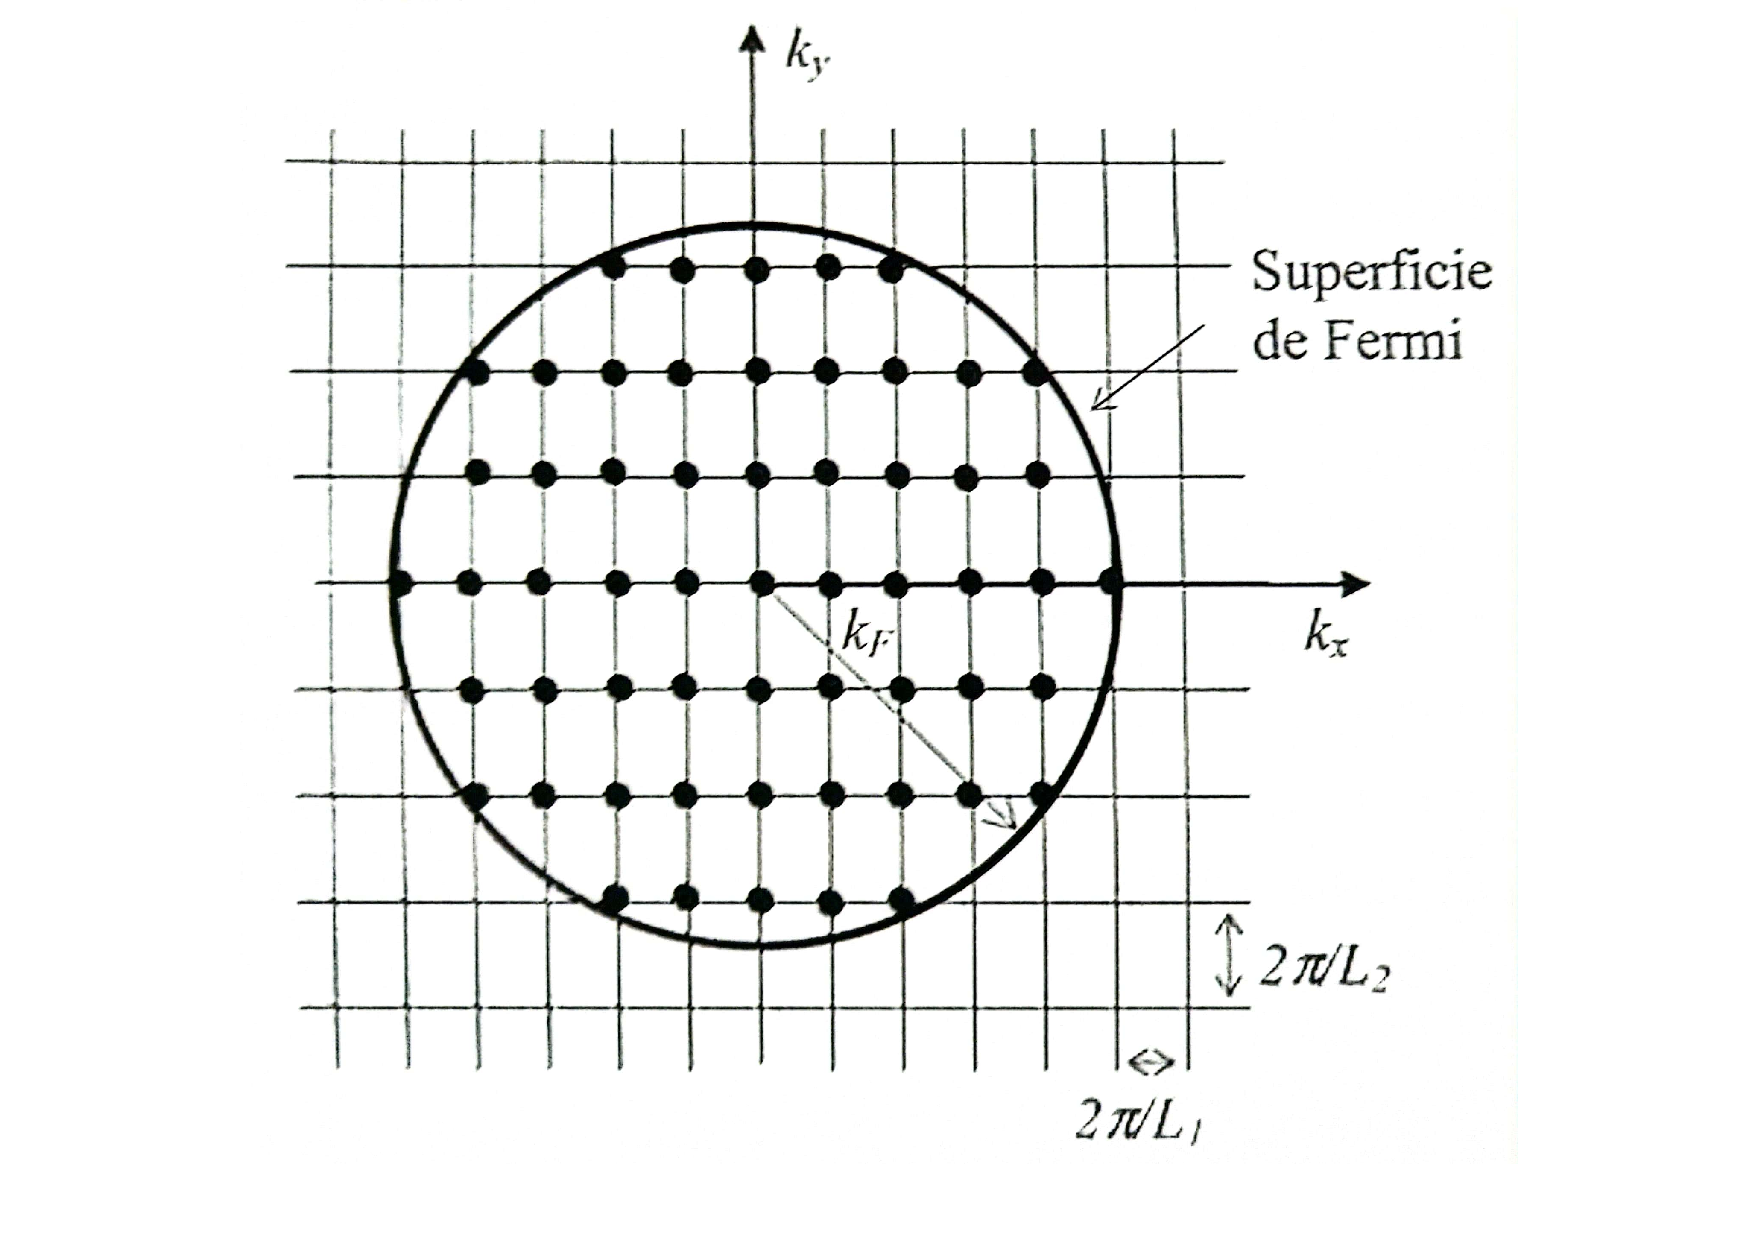
\includegraphics[scale=0.35]{Cuerpo/Ch_06/Fotos libro 1.pdf}
    \caption{Distribución de estados electrónicos ocupados en el espacio de fases.}
    \label{Fig:06-01}
\end{figure}    

La \textit{superficie de Fermi} es la superficie que separa los estados ocupados de los desocupados. A continuación vamos a definir los términos de Fermi:

\begin{itemize}
	\item \textbf{Vector de onda de Fermi (3D):}
	\begin{equation}
		k_F = (3\pi^2 n)^{1/3} \quad (n\equiv N/V) \label{Ec:06-01-05}
	\end{equation}
	\item \textbf{Vector de onda de Fermi (2D):}
	\begin{equation}
		k_F= \sqrt{2\pi n}
	\end{equation}
	\item \textbf{Energía de Fermi:}
	\begin{eqnarray}
		\varepsilon_F \equiv \frac{\hbar^2 k_F^2}{2m} \label{Ec:06-01-07}
	\end{eqnarray}
	\item \textbf{Velocidad de Fermi:}
	\begin{eqnarray}
	v_F \equiv \sqrt{2\varepsilon_F /m}
	\end{eqnarray}
	\item \textbf{Temperatura de Fermi:}
	\begin{eqnarray}
		T_F \equiv k_B \varepsilon_F
	\end{eqnarray}
\end{itemize}
Todos estos parámetros dependen sólo de la concentración electrónica $n$ uqe es conocida para metales: $10^{22}<n(\textbf{cm}^{-1})<10^{23}$. Numéricamente, resultan los siguientes valores:

\begin{equation*}
	\begin{array}{c}
	\varepsilon_F = 1-10 \unit{\eV} \\
	T_F = 10^4 - 10^5 \unit{K} \\
	v_F = (0.7-2)\times 10^8 \unit{\cm/s}\\
	v_F = (0.7-1.7)\times 10^8 \unit{\cm^{-1}}
	\end{array}
\end{equation*}
La \textbf{densidad de estados} $D(\varepsilon)$ se calculaa fácilmente haciendo referencia a la figura \ref{Fig:06-02}, resultando:

\begin{equation}
	D(\varepsilon) \D \varepsilon = 2 \times \frac{4\pi k^2 \D k}{8 \pi3 /V} = \frac{V}{2\pi2} \parentesis{\frac{2m}{\hbar2}}^{3/2} \sqrt{\varepsilon} \D \varepsilon \label{Ec:06-01-10}
\end{equation}
El factor $2$ da cuenta de los dos estados electrónicos posibles. Es útil expresar la densidad de estados $D(\varepsilon)$ en función de $\varepsilon_F$ combinando (\ref{Ec:06-01-10}), con (\ref{Ec:06-01-05}) y (\ref{Ec:06-01-07}) resulta:

\begin{equation}
	D(\varepsilon) = \frac{3}{2} \frac{N}{\varepsilon_F} \sqrt{\frac{\varepsilon}{\varepsilon_F}} \label{Ec:06-01-11}
\end{equation}	

A menudo es más útil trabajar con el número de estados por unidad de volumen del cristal, en cuyo caso basta hacer en (\ref{Ec:06-01-12}) la sustitución $N\rightarrow N/V=n$.
	
\begin{figure}[h!] \centering
    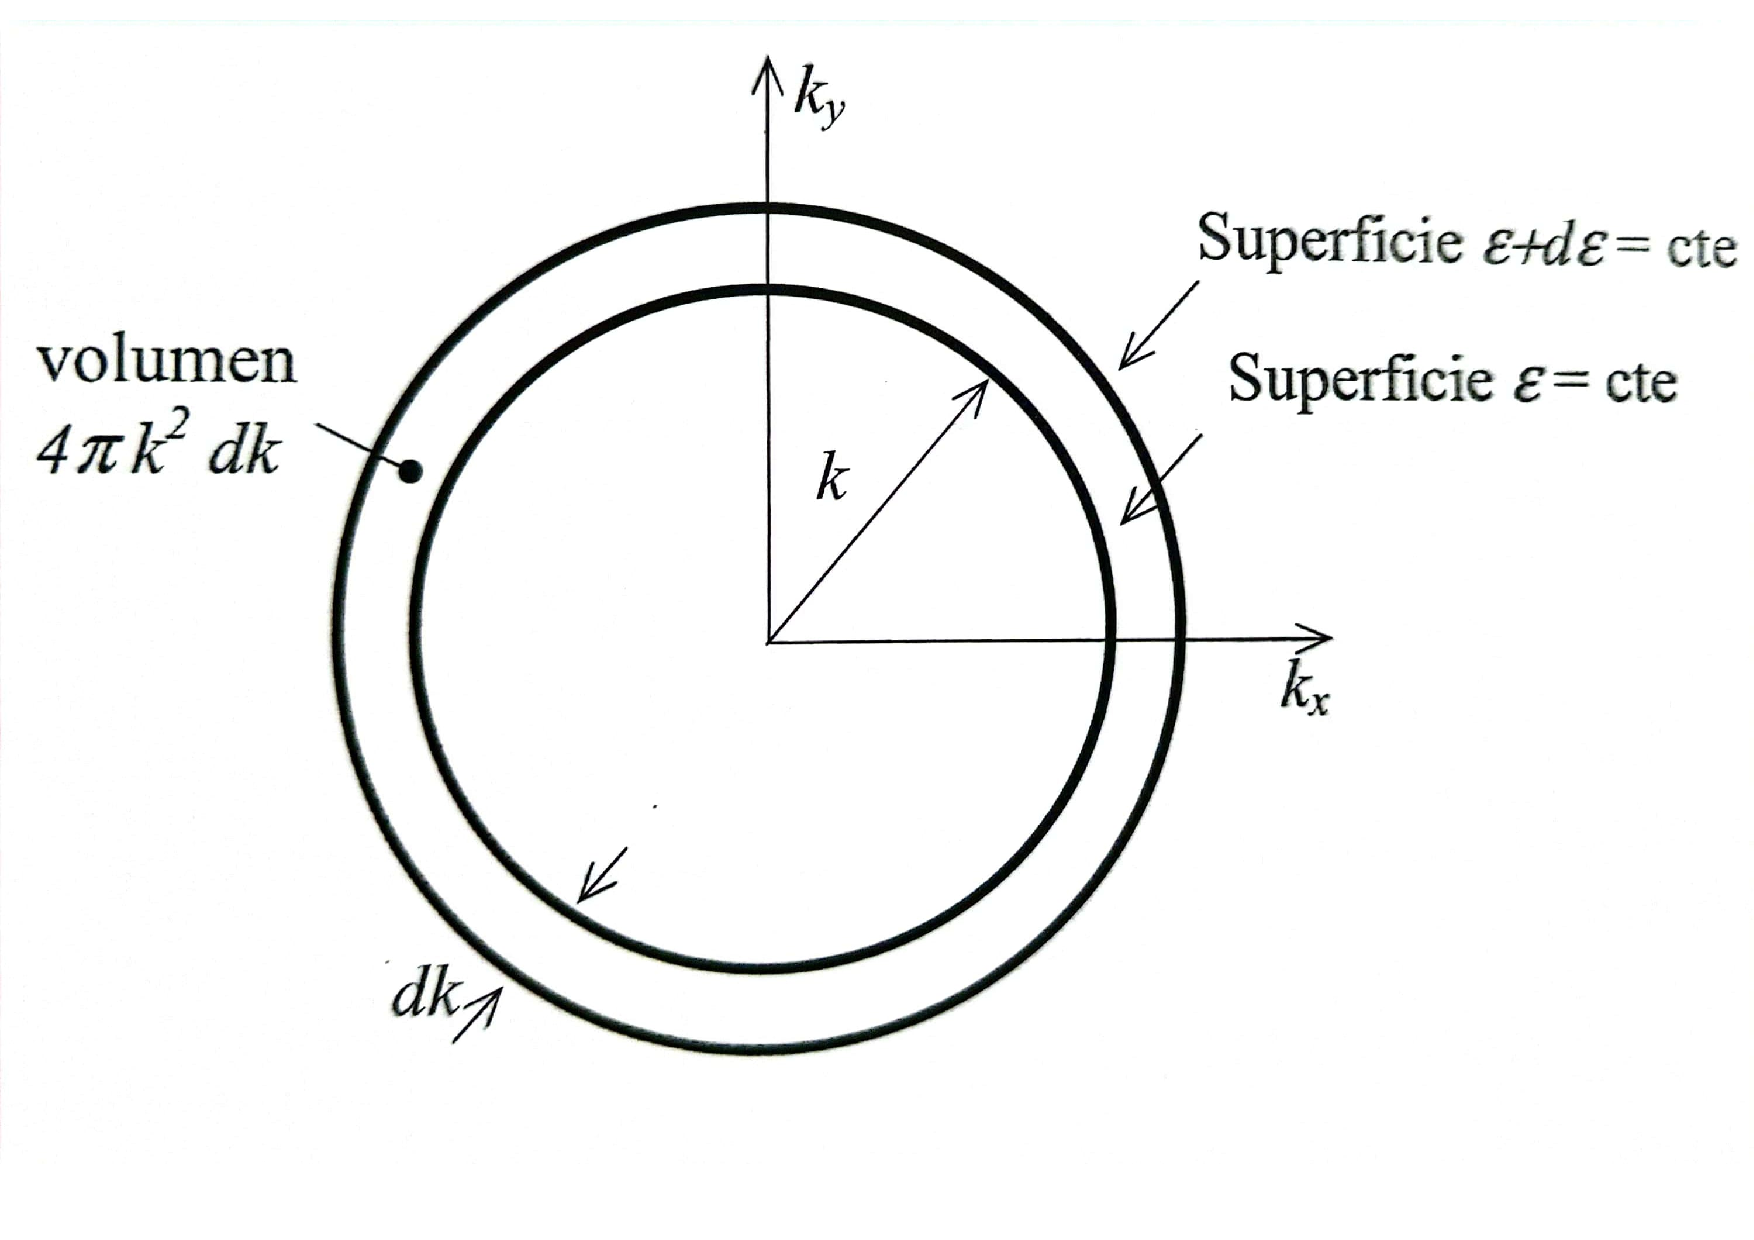
\includegraphics[scale=0.35]{Cuerpo/Ch_06/Fotos libro 2.pdf}
    \caption{Cálculo de la densidad de estados electrónicos.}
    \label{Fig:06-02}
\end{figure}  

\subsection{Ocupación de estados a $T>0$}

Se trata de saber cómo cambia el llenado de estados si el gas de electrones está a una temperatura finita. Por tratase de fermiones la respuesta la da la distribución de Fermi-Dirac, según la cual la probabilidad $f_{FD}$ de que un estado $\kn$ esté ocupado es:

\begin{equation}
	f_{FD} (\kn) = \frac{1}{e^{(\varepsilon(\kn)-\mu)/k_B T} +1}  \label{Ec:06-01-13}
\end{equation}
donde $\mu$ es el potencial química que verifica $f_{FD}(\mu)=1/2$. A $T=0$K, como esperaríamos, $f_{FD}(\varepsilon<\mu)=1$ y $f_{FD}(\varepsilon>\mu)=0$, por lo que podemos decir que $\varepsilon_F=\mu(T=0\textbf{K})$. A $T>0$ K la función $f_{FD}$ tiene el perfil que se grafíca en la figura \ref{Fig:06-03}. El potencial químico de la ligadura:

\begin{equation}
	N=\int_0^{\infty} f_{FD} (\varepsilon) D (\varepsilon) \D \varepsilon  \label{Ec:06-01-14}
\end{equation}
Al sustituir (\ref{Ec:06-01-11}) y (\ref{Ec:06-01-13}) en (\ref{Ec:06-01-14})  resulta una integral no analítica. Gracias a que $T\ll T_F$ las integrales de tipo (\ref{Ec:06-01-14}) se pueden aproximar por la llamada \textit{expansión de Sommerfeld} 

\begin{eqnarray}
	\int_{0}^{\infty} H(\varepsilon) f_{FD} (\varepsilon)  \D \varepsilon \approx \int_0^\mu H(\varepsilon) \D \varepsilon + \frac{\pi2 k_B^2 T^2}{6} \derivadas{\D H}{\D \varepsilon} (\mu)
\end{eqnarray}
Aplicando esta relación a (\ref{Ec:06-01-14}), tras alguna manipulación se llega a 

\begin{equation}
	\mu (T) = \mu(0) \ccorchetes{1-\frac{1}{3} \parentesis{\frac{\pi T}{2 T_F}}^2}
	\label{Ec:06-01-15}
\end{equation}
Usando los valores característicos para $T_F$, la lectura  de (\ref{Ec:06-01-15}) es que para que metales, incluso a la temperatura ambiente, se puede aproximar $\mu (T) \approx \varepsilon_F$ dentro del $0.01\%$, y concluimos que el gas electrónico resulta sólo muy ligeramente alterado de $T=0$ K a $T\sim 300$ K. Por tanto, en muchos casos se podrá aproximar la energía total a cualquier temperatura:

\begin{equation}
	U(T) = \int_0^\infty \varepsilon D(\varepsilon) f_{FD} \D \varepsilon 
\end{equation}
por la correspondiente a $T=0$ K (energía del punto cero):

\begin{equation}
	U(0) = \int_0^{\varepsilon_F} \varepsilon D(\varepsilon) \D \varepsilon
\end{equation}
pues $f_{FD}(\varepsilon,T)=1$ para $\varepsilon\leq\varepsilon_F$ y $f_{FD} (\varDelta,T)=0$ para $\varepsilon>\varepsilon_F$. Si sustituimos (\ref{Ec:06-01-11})	en la anterior expresión e integramos se obtiene:

\begin{equation}
	U(0)=\frac{3}{5} N \varepsilon_F
\end{equation}
de modo que la energía por electrón es, por (\ref{Ec:06-01-07}):

\begin{equation}
	u(0)=\frac{3}{5} \varepsilon_F = \frac{3}{5} \parentesis{\frac{\hbar^2 k_F^2}{2m}} = \frac{3\hbar^2}{10m} (3 \pi^2 n)^{2/3}
\end{equation}
que es la energía que fue utilizada al tratar el enlace metálico.


\begin{figure}[h!] \centering
    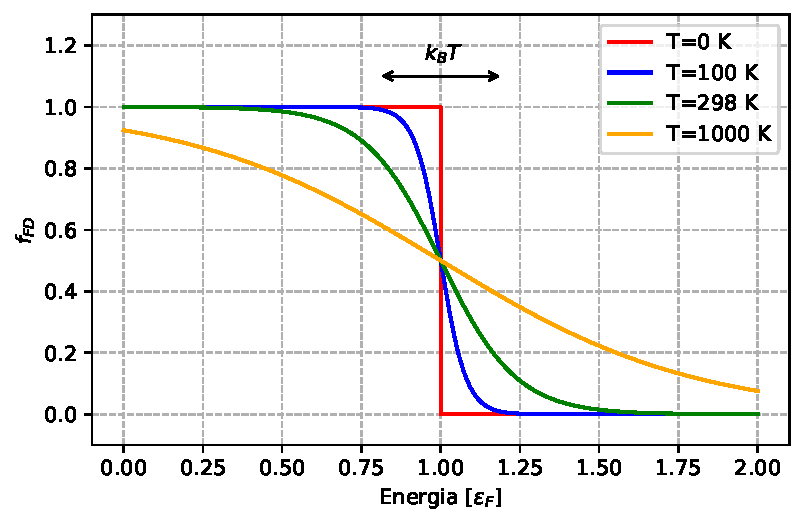
\includegraphics[scale=0.75]{Cuerpo/Ch_06/06-Fermi-Dirac.pdf}
    \caption{Distribución de Fermi-Dirac.}
    \label{Fig:06-03}
\end{figure}    

\subsection{Interacción electrón-electrón}

Es un metal la distancia media entre electrones de conducción es del orden de unos pocos $\unit{\angstrom}$ y, sin embargo, los recorridos libres medios para las colisiones elcetrón-electrón son mayores que $10^4 \unit{\angstrom}$ a temperatura ambiente, y superiores a 10 cm a 1 K. Uno de los factores responsables de esta falta de interacción entre electrones y que justifica la aproximación de electrones independientes es el Principio de Exclusión.

\begin{figure}[h!] \centering
    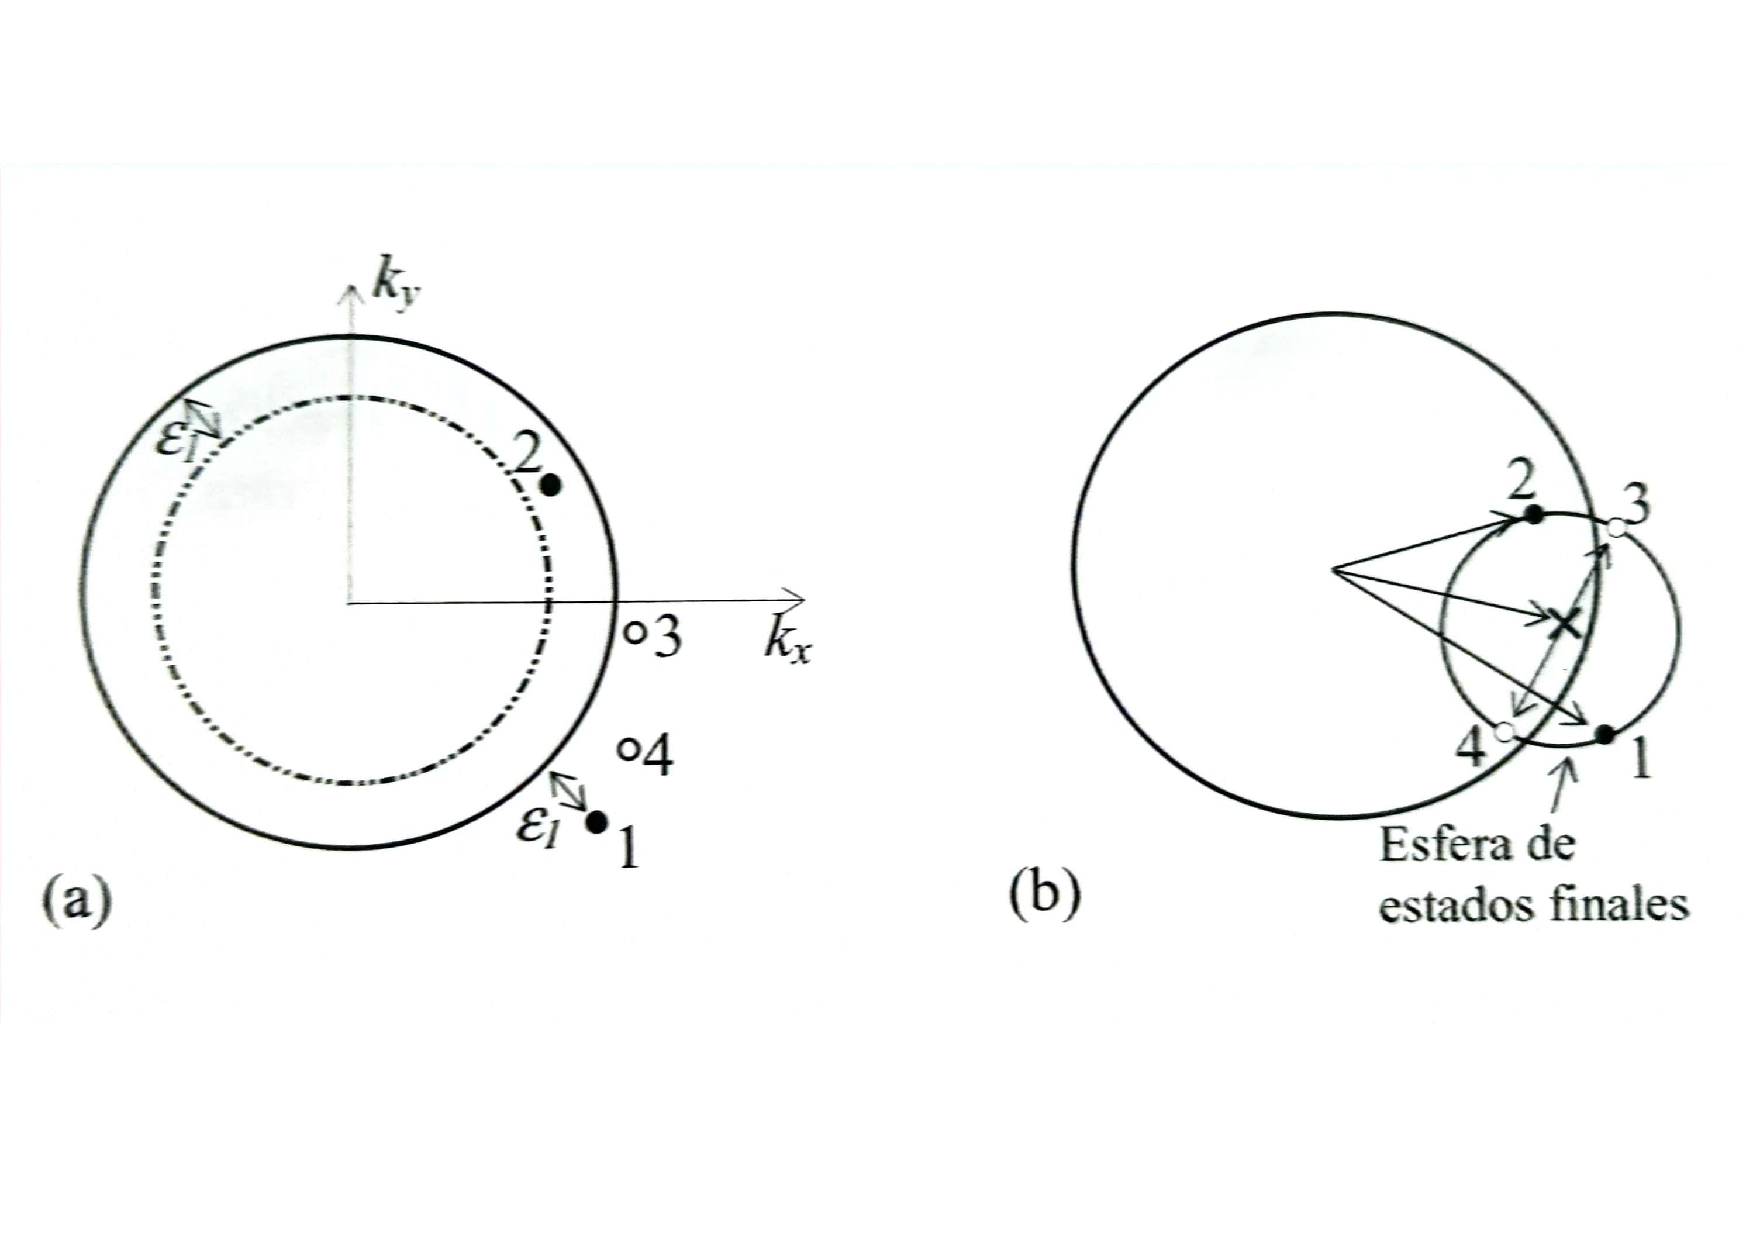
\includegraphics[scale=0.35]{Cuerpo/Ch_06/Fotos libro 4.pdf}
    \caption{Restricción a los procesos de colisión $e^- - e^-$ debido a las leyes de conservación de la energía (a) y del momento (b).}
    \label{Fig:06-04}
\end{figure}  

Consideremos la situación especialmente sencilla de una esfera de Fermi con un solo electrón excitado 1 con energía $\varepsilon_1$ respecto del nivel de Fermi. Como ilustra la figura \ref{Fig:06-04} (a), no todos los electrones 2 pueden colisionar con el 1, de modo que $1+2\rightarrow3+4$, pues los estados finales 3 y 4 deben estar desocupados. La condición $\varepsilon_3 + \varepsilon_4 = \varepsilon_1 + \varepsilon_2$ exige $|\varepsilon_2|<\varepsilon_1$ por lo que sólo una fracción $\sim \varepsilon_1 / \varepsilon_F$ de los electrones totales constituye un blanco para el electrón 1. La condición $\kn_1 + \kn_2 = \kn_3 + \kn_4$ limita aún más los estados finales: deben caer en la esfera de estados finales que ilustra la figura \ref{Fig:06-04} (b), y fuera del mar de Fermi la fracción permitida resulta ser también $\sim \varepsilon_1 / \varepsilon_F$. El producto de las dos fracciones es $\sim (\varepsilon_1/\varepsilon_F)^2$. 
En presencia de una temperatura finita puede equipararse $\varepsilon_1$ con $k_BT$, con lo que el Principio de Exclusión reduce las colisiones electrón-electrón en un factor $\sim (k_BT/\varepsilon_F)^2 \sim 10^4$. El correspondiente recorrido libre a temperatura ambiente es $\sim 10^4 \ \unit{\angstrom}$, mucho mayor que el debido a la interacción electrón-fonón.

\section{Capacidad térmica electrónica}

La contribución electrónica a la capacidad térmica medida en metales es $\sim 1\%$. Si los electrones fueran partículas clásicas la capacidad debería ser $\frac{3}{2} N k_BT$ y la energía que ganan $\sim k_B T$. Así pues $U(T) \approx U(0)+\frac{3N}{2\varepsilon_F} k_B^2 T^2$ y entonces

\begin{eqnarray}
	C_{el} \approx 3 N k_B \frac{T}{T_F}
\end{eqnarray}
que es directamente proporcional a $T$, de acuerdo con los resultados experimentales, y mucho menor que el valor clásico $\frac{3}{2} Nk_B$  debido a que $T\ll T_F$. El cálculo más formal se realiza a partir de $U=\int_{0}^{\infty} \varepsilon D(\varepsilon) f_{FD} (\varepsilon) \D \varepsilon$ que, vía la expansión de Sommerfeld, conduce a 

\begin{eqnarray}
	C_{el} = \frac{\pi^2}{2} N k_B \frac{T}{T_F}
\end{eqnarray}
La medida de la capacidad térmica electrónica debe hacerse a muy bajas temperaturas para no ser enmascarada por la contribución de la red (que es proporcional a $T^3$ cuando $T\rightarrow 0$). La dependencia lineal con $T$ se verifica excelentemente, pero de acuerdo del coeficiente $\gamma$ en $c_{el} = \gamma T$ es, como ilustra la tabla \ref{Tab:06-01}, muy variable y en algunos casos muy alejado del valor experimental.

\begin{table}[h!] \centering
	\begin{tabular}{cccc} 
		Elemento & $\gamma_{\text{el.libres}}$ &  $\gamma_{\text{exp}}$ & cociente \\
 		& ($10^{-4} \frac{\text{cal}}{\text{mol}\cdot\text{K}^2}$) & ($10^{-4} \frac{\text{cal}}{\text{mol}\cdot\text{K}^2}$)  &  \\ \hline
 		Li & 1.8 & 4.2 & 2.3 \\
 		Na & 2.6 & 3.5 & 1.3 \\
 		Cs & 5.3 & 7.7 & 1.5 \\
 		Cu & 1.2 & 1.6 & 1.3 \\
 		Au & 1.5 & 1.6 & 1.1 \\
 		Sr & 4.3 & 8.7 & 2.0 \\
 		Fe & 1.5 & 12 & 8.0 \\
 		Zn & 1.8 & 1.4 & 0.78 \\
 		Pb & 3.6 & 7.0 & 1.9 \\
 		Bi & 4.3 & 0.2 & 0.047 
	\end{tabular}	
	\caption{Predicción de la teoría de $e^-$ libres y resultado experimental para el coeficiente $\gamma$ de distintos elementos.}
	\label{Tab:06-01}
\end{table}

\section{Conductividad eléctrica DC}

Los otros metales se caracterizan por una alta conductividad eléctrica, $\sigma$, comparada con otros materiales [$10^8$-$10^7$ ($\Omega$m)$^{-1}$ frente a $10^5$-$10^{-4}$ ($\Omega$m)$^{-1}$ en semiconductores y hasta $10^{-16}$ ($\Omega$m)$^{-1}$ en aislantes]. Electrones completamente libres e independientes (es decir, no interaccionantes con la red o entre ellos) darían lugar a una conductividad eléctrica infinita. Se introduce por tanto un modelo cinético similar al utilizado en el capítulo \ref{Ch:05} con fonones, según el cual los electrones colisionan con una probabilidad de tiempo $\tau^{-1}$ con fonones, defectos reticulares y en menor medida con otros electrones (\textit{modelo de Drude}). En este modelo cinético los electrones se tratan clásicamente. Esto es posible porque podemos formar, a partir de las funciones de onda (\ref{Ec:06-01-01}), un paquete de ondas de extensión espacial $\Delta x$ verificando $\Delta k \Delta x \sim 1$. Como $\Delta k$ debe estar bien definido, es decir $\Delta k \ll k_F \sim a^{-1}$, debe ser $\Delta x \gg a$. Por tanto, el modelo será aplicable siempre que las características de posibles perturbaciones (la longitud de onda de campos aplicados o el recorrido libre medio, ver más abajo) sean mucho mayores que $a$. 

Para obtener una ecuación dinámica para los electrones colisionantes, supongamos que $\pn(t)= m \vn(t)$ es el impulso medio de la colectividad de electrones y $\fn(t)$ la fuerza media. Si se sigue la evolución del gas de $t$ a $t+\D t$ se tiene:

\begin{equation}
	\pn (t+\D t) = \parentesis{1-\frac{\D t}{\tau}} \ccorchetes{\pn(t)+\fn(t)\D t} + o(\D t^2)
\end{equation}
donde se ha restado el impulso de las $\D t/\tau$ partículas que han colisionado en el intervalo $\D t$. Teniendo en cuenta que $\pn(t+\D t)=\pn(t)+(\D \pn / \D t)\D t$, la relación anterior conduce inmediatamente a 

\begin{equation}
	\derivadas{\pn(t)}{t} \equiv - \frac{\pn(t)}{\tau} +  \fn(t)	
\end{equation}


\subsection{Modelo cinético de Drude y ecuación dinámica}

\subsection{Ley de Ohm}
\begin{figure}[h!] \centering
    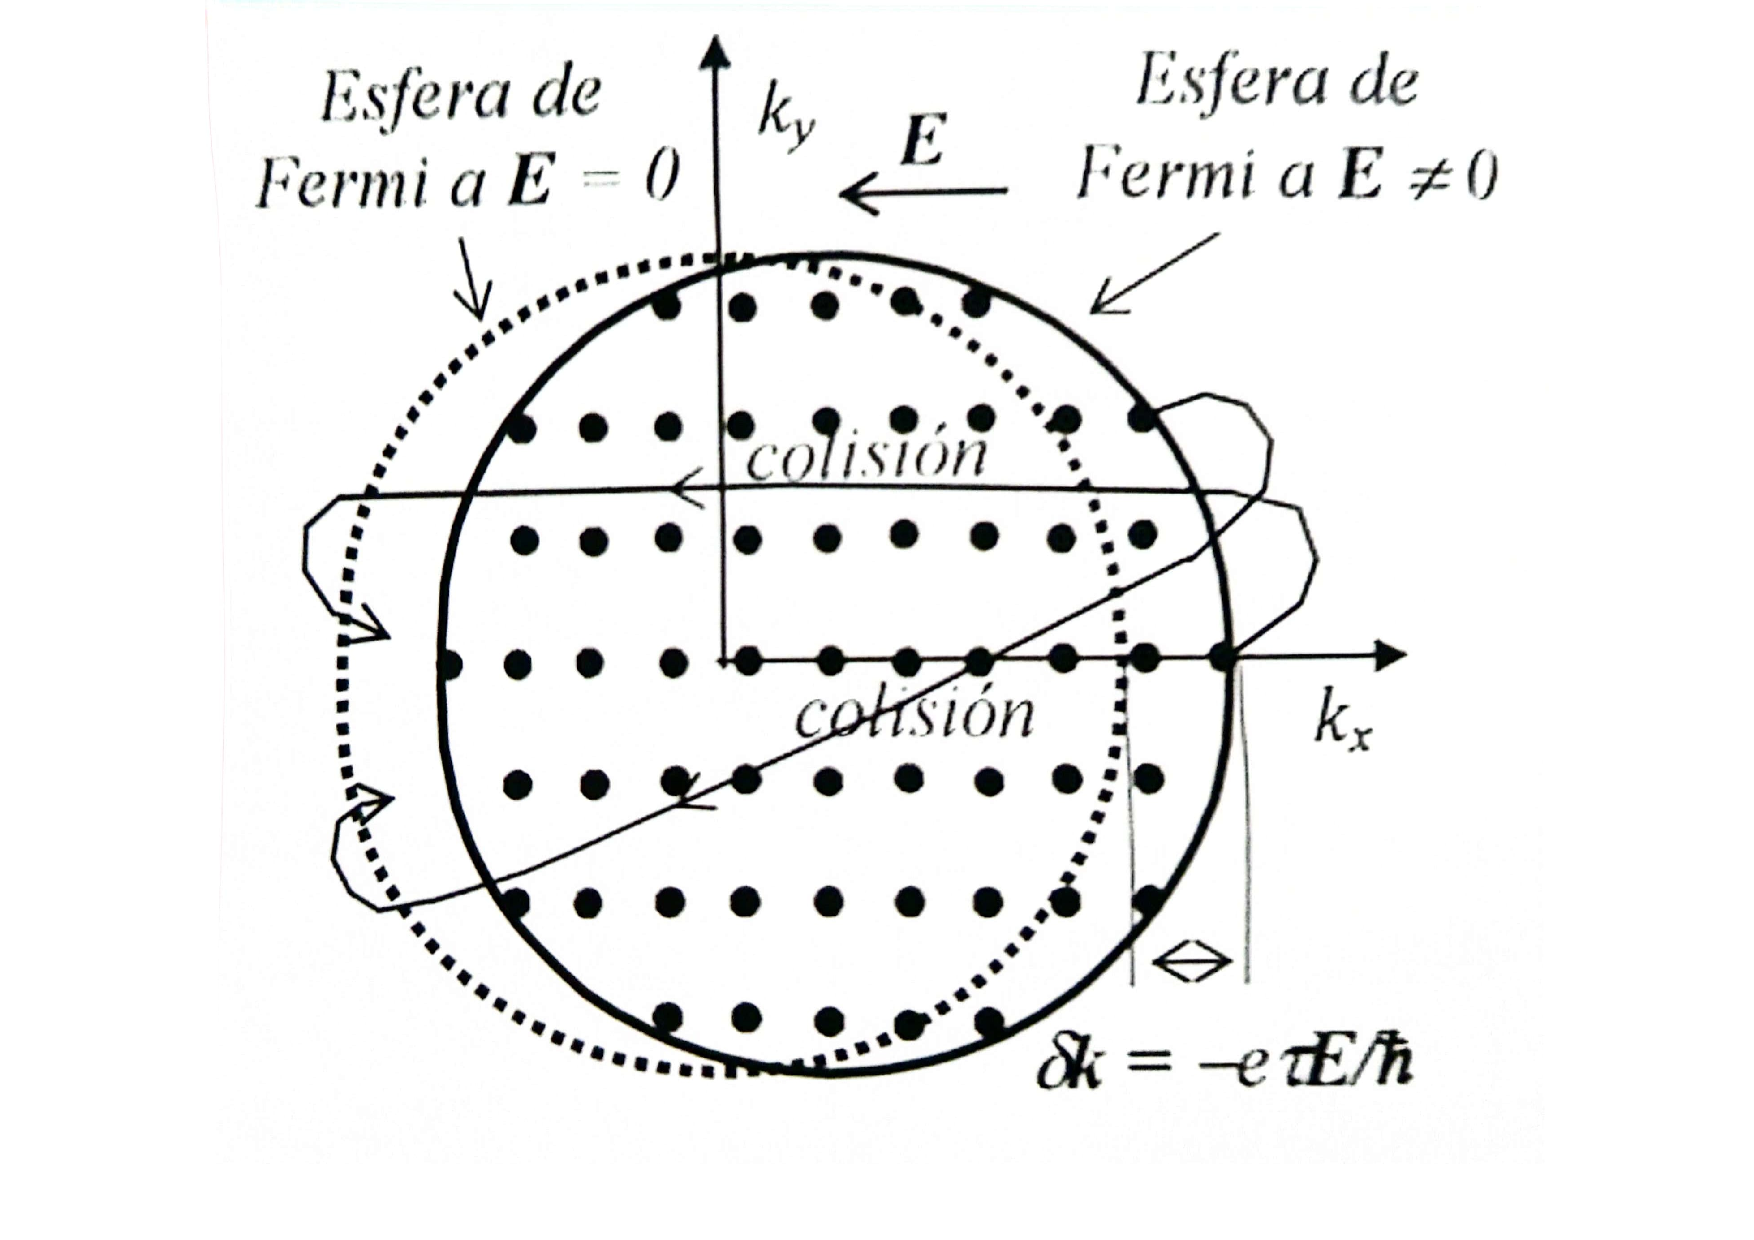
\includegraphics[scale=0.5]{Cuerpo/Ch_06/Fotos libro 5.pdf}
    \caption{Desplazamiento de la ``esfera de Fermi'' bajo la aplicación de un campo eléctrico. Las líneas indican algunos procesos de colisión permitidos.}
    \label{Fig:06-05}
\end{figure}  

\subsection{Dependencia con la temperatura de la conductividad eléctrica}
\begin{figure}[h!] \centering
    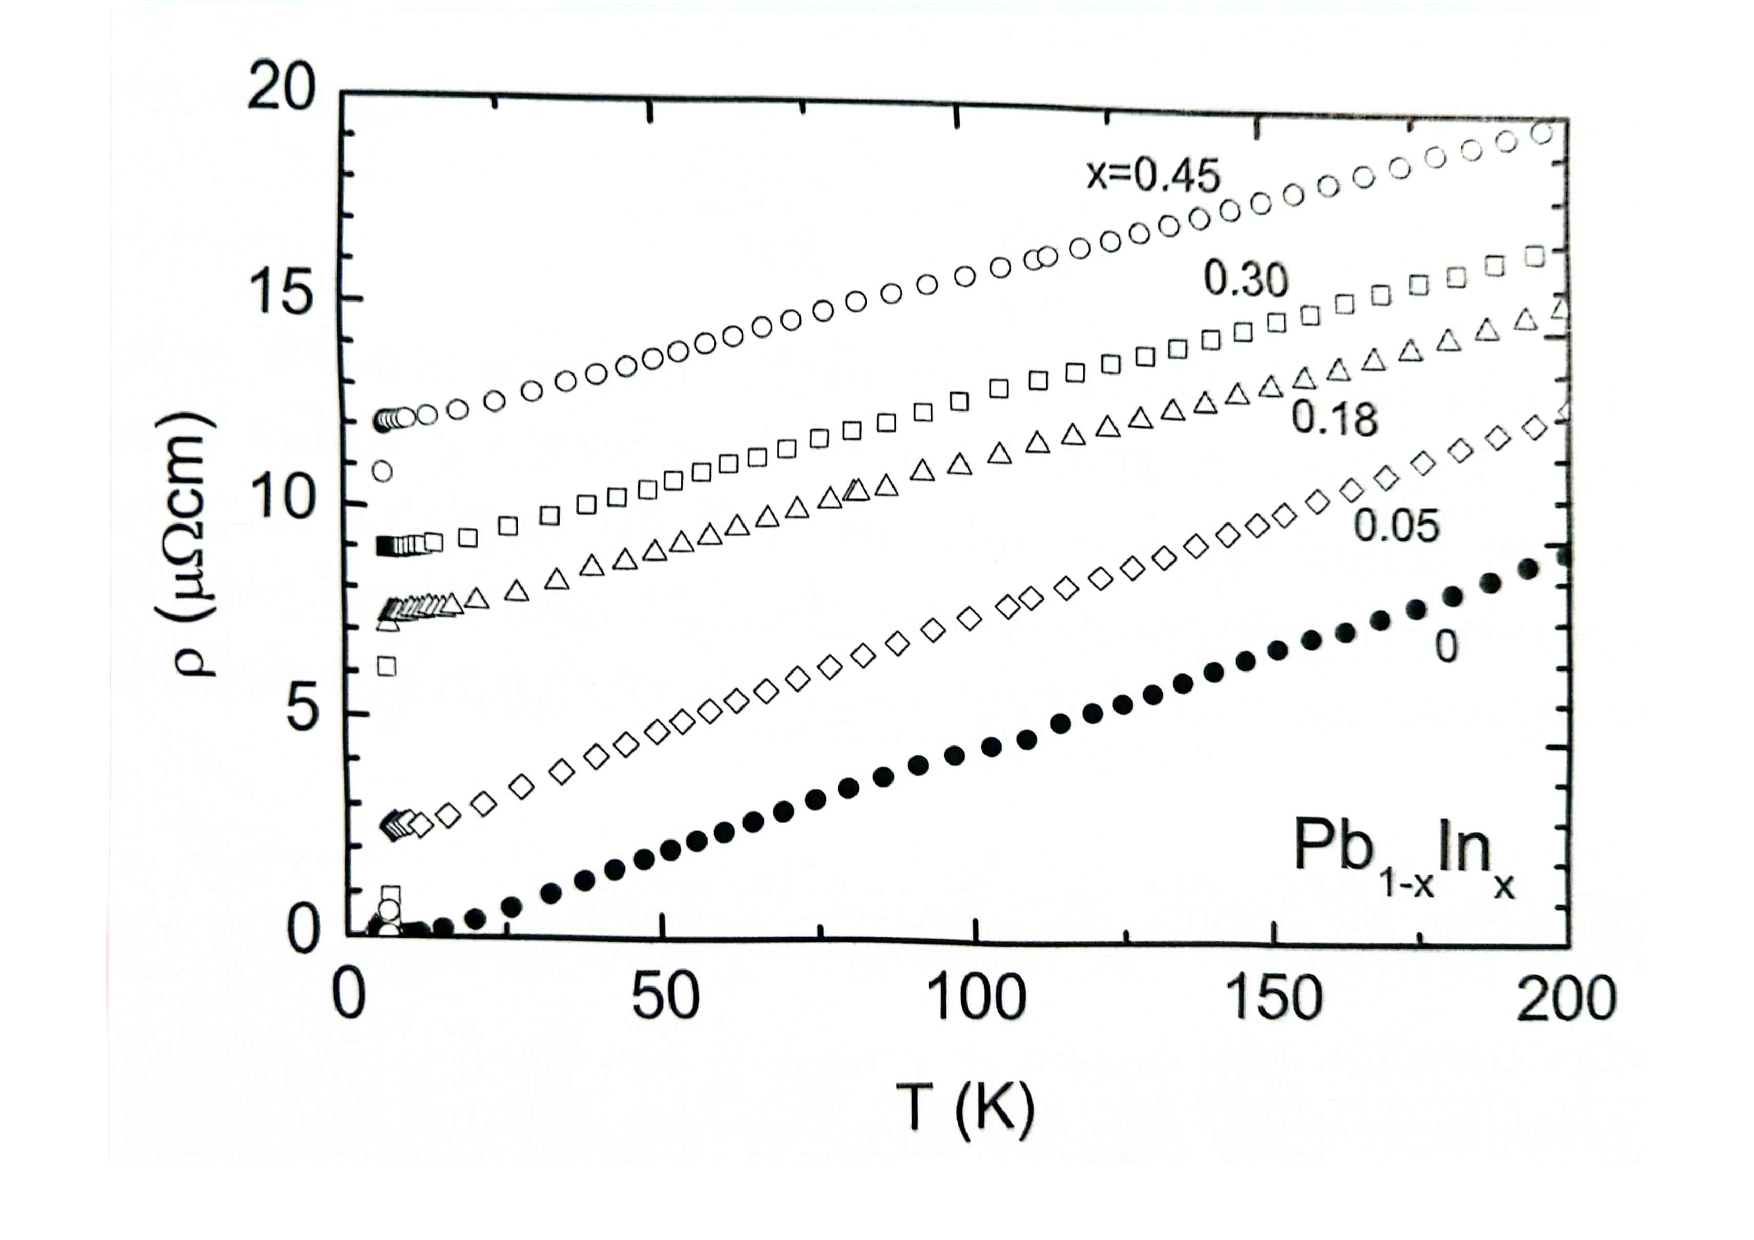
\includegraphics[scale=0.5]{Cuerpo/Ch_06/Fotos libro 6.pdf}
    \caption{Comprobación de la regla de Mathiessen con la resistividad de aleaciones de Pb-In. Al aumentar $x$ el desorden de la aleación y por tanto la contribución constante $\rho_{\text{def}}$ frente a $\rho_{\text{fon}} (T)$ que casi no cambia (nótese que la pendiente no varía). Es interesante que estas aleaciones son superconductores por debajo de $\sim 7$ K (veáse Capítulo \ref{Ch:11}).}
    \label{Fig:06-06}
\end{figure}  


\section{Conductivdad térmica electrónica}



\section{Ley de Wiedmann-Franz}

\section{Efecto Hall y magnetorresistividad}
\begin{figure}[h!] \centering
    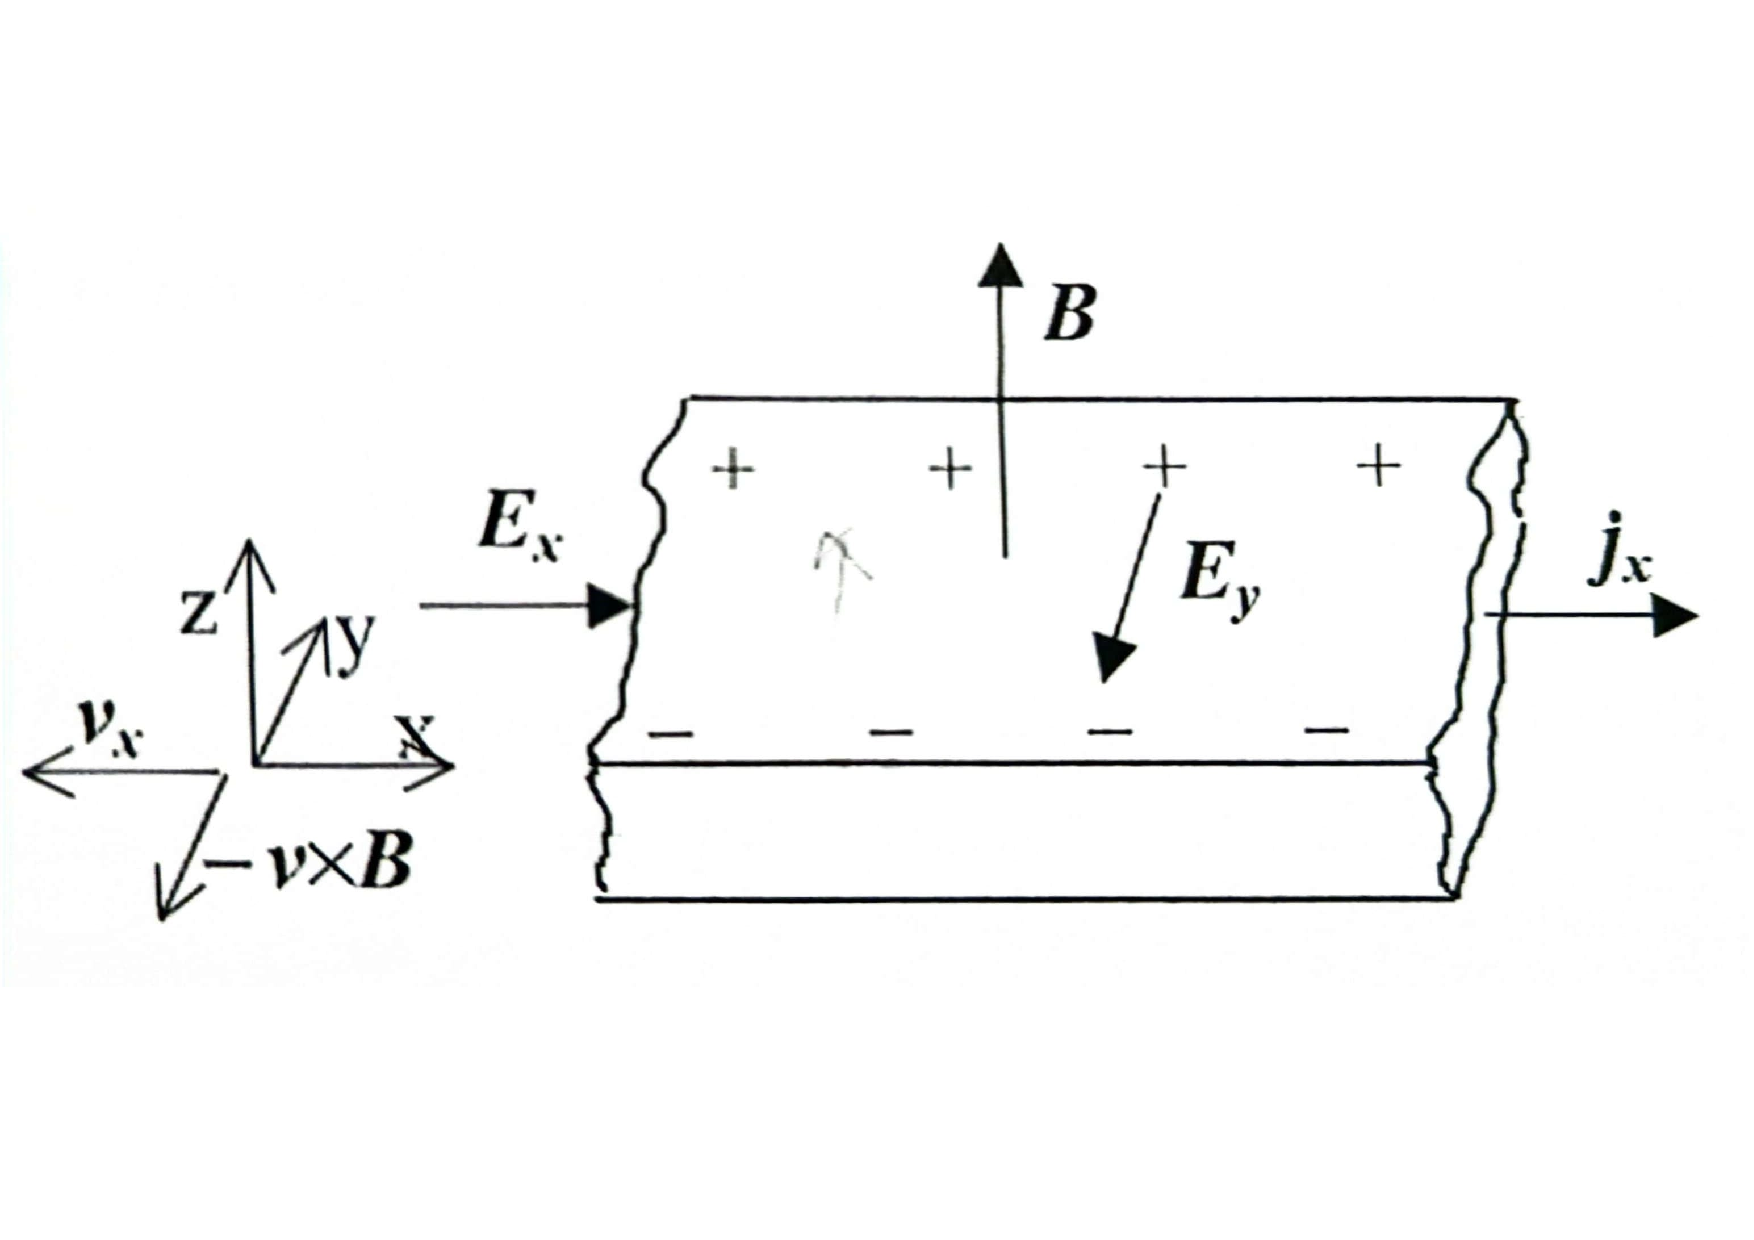
\includegraphics[scale=0.5]{Cuerpo/Ch_06/Fotos libro 7.pdf}
    \caption{Configuración experimental para comprobar el efecto Hall.}
    \label{Fig:06-07}
\end{figure}  


\section{Conductividad AC y propiedades ópticas}
